% Tikz File 'mytikz.tex'
\documentclass{standalone}
\usepackage{tikz}
%\usetikzlibrary{...}
\begin{document}
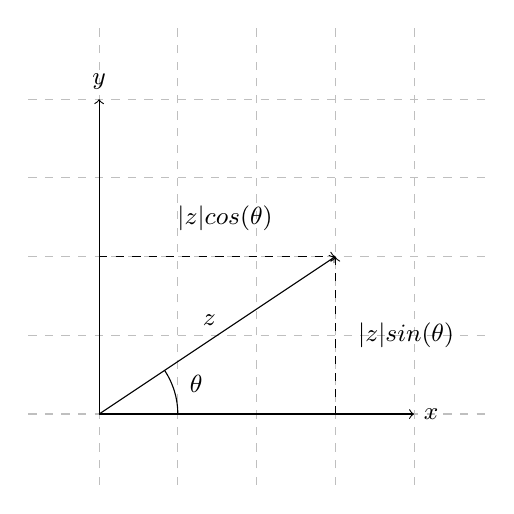
\begin{tikzpicture}
  % Add grid
  \draw[gray!50, dashed, step=1] (-0.9,-0.9) grid (4.9,4.9);

  % Draw the sine function

  % Add axes
  \draw[->] (0,0) -- (4,0) node[right] {\small $x$};
  \draw[->] (0,0) -- (0,4) node[above] {\small $y$};

  \draw[->] (0,0) -- (3, 2) node[above, xshift=-1.6cm, yshift=-1cm] {\small $z$};

  \draw[->, black, dashed] (3, 0) -- (3, 2) node[above, yshift=-1.28cm, xshift=0.9cm] {\small $|z|sin(\theta)$};

  \draw[->, black, dashed] (0, 2) -- (3, 2) node[above, yshift=0.2cm, xshift=-1.4cm] {\small $|z|cos(\theta)$};

  \draw (1,0) arc (0:33.69:1) node[above, yshift=-0.4cm, xshift=0.4cm] {\small $\theta$};

\end{tikzpicture}
\end{document}


